%!TEX root = ../../csuthesis_main.tex
\chapter{基于通道注意力机制的CORnet-Z模型优化}

\section{引入注意力机制的动因}

\subsection{生物学基础:神经皮层的选择性响应}

在前述CORnet-S和CORnet-Z的模型结构中,各模块的特征提取过程采用标准卷积网络设计,未显式引入注意力调节机制。虽然该类模型在识别准确率与类脑性评估方面已具备一定表现,但在应对复杂图像背景、多目标干扰及特征稀疏性等问题时,模型关注能力有限,存在信息利用不足与干扰区域激活过强的问题。为此,本文在CORnet-Z模型基础上引入通道注意力机制,以增强模型对关键信息通道的响应能力,提高其表示效率与抗干扰性。

在生物视觉系统中,注意力机制是一种重要的资源调控方式。神经科学研究表明,视觉注意不仅体现在空间定位上,更作用于通道层面上的信息筛选。例如在初级视觉皮层(V1)、中层(V4)和高层(IT)区域,不同神经元对颜色、方向、边缘、轮廓等特征的响应存在显著选择性。当注意力被引导至特定目标时,相关通道的神经活动显著增强,而无关通道则受到抑制(Desimone Duncan, 1995)。

这种选择性响应机制被认为有助于大脑在有限神经资源条件下提高感知效率和行为反应速度。类脑视觉模型若能模拟这一神经调节行为,将有望提升其在复杂环境中的识别稳健性和神经表征一致性。

SE(Squeeze-and-Excitation)模块的提出正是基于类似生物动因。该模块通过压缩(squeeze)操作捕获全局通道信息,并通过激励(excitation)机制计算各通道的重要性得分,实现对特征通道的重新加权,有助于模拟大脑对关键通道信号的增强调节过程。

\subsection{工程动因:特征表示稀疏性与判别性}

从工程实践角度看,传统CNN模型在特征提取过程中常存在部分通道响应冗余、不具判别性的问题,尤其是在浅层网络结构中更为显著。模型若对所有通道一视同仁,容易在训练过程中浪费计算资源,并在推理时产生对背景噪声的错误响应,影响分类准确率和泛化能力。

引入通道注意力机制可以实现特征通道的“压缩筛选”,使模型在保持原有结构深度不变的前提下增强关键特征的表达能力,并压制冗余和干扰信号。SE模块作为一种轻量级注意力机制,不引入额外空间维度,也不显著增加模型参数量,适合嵌入至CORnet-Z这类轻量网络结构中。

在多类目标混合、背景复杂的Tiny-ImageNet数据集上,特征表示的有效性对于模型分类表现尤为关键。通过在CORnet-Z的V4或IT层引入SE模块,模型能够在高层语义表示阶段加强对目标核心区域的响应,从而提高模型在Top-1、Top-5准确率方面的性能表现,也为后续类脑性对齐实验提供结构基础。

\section{通道注意力模块设计与集成}

\subsection{SE结构原理与实现}

为增强CORnet-Z模型在图像识别过程中的通道选择能力,本文在原始模型结构的基础上引入Squeeze-and-Excitation(SE注意力模块,构建了改进模型CORnet-Z+SE。该机制通过显式建模通道之间的依赖关系,实现对冗余特征的压制与有效特征的增强,从而提升模型的判别能力与可解释性。

SE模块由Hu等人于2018年提出,核心思想是通过两个阶段实现特征通道的重要性建模:squeeze(压缩)与 excitation(激励)。

在 squeeze 阶段,模块对输入特征图的每个通道进行全局平均池化,得到一个通道描述向量,压缩掉空间维度:

\begin{equation}
	z_c = 
	\frac{1}{H \times W} 
	\sum_{i=1}^{H} \sum_{j=1}^{W} x_c(i, j)
	\label{eq:se_squeeze}
\end{equation}

其中,$x_c(i,j)$表示输入特征图第$c$个通道在位置$(i,j)$的值,$z_c$为池化后通道$c$的全局描述,$H$和$W$分别为特征图的空间尺寸。

在excitation阶段,该通道向量$z$经过一个由两个全连接层组成的非线性变换,输出通道注意力权重向量$s$:

\begin{equation}
	s = \sigma \left( W_2 \cdot \text{ReLU} \left( W_1 \cdot z \right) \right)
	\label{eq:se_excitation}
\end{equation}

其中,$W_1 \in \mathbb{R}^{\frac{C}{r} \times C}$和$W_2 \in \mathbb{R}^{C \times \frac{C}{r}}$是两层全连接层的权重矩阵,$r$为压缩比超参数,用于控制中间层维度大小;$\text{ReLU}(\cdot)$表示线性整流函数,$\sigma(\cdot)$ 为Sigmoid 激活函数,用于将权重归一化到$[0,1]$区间。

最后,将注意力权重向量$s$与原始特征图逐通道相乘,完成对输入特征的加权重标定:

\begin{equation}
	\tilde{x}_c = s_c \cdot x_c
	\label{eq:se_scale}
\end{equation}

其中,$\tilde{x}_c$表示重标定后的通道特征图,$s_c$为通道$c$的注意力系数。通过这一机制,SE模块能够提升模型对目标区域特征的响应能力,增强判别特性。

在本文的实现中,使用PyTorch编写的\texttt{SEBlock}类对上述结构进行了复现。池化操作采用\texttt{nn.AdaptiveAvgPool2d(1)},全连接层使用两层\texttt{Linear}模块分别对应压缩与激励过程,激活函数为ReLU和Sigmoid。参数初始化方面,前层使用\texttt{kaiming\_normal\_},后层采用\texttt{normal\_}方法,以保证训练初期的稳定性。不同于原始论文中默认的压缩比$r=16$,本文选用更小的压缩比$r=8$,以减小信息损失并提高特征保持能力,使模块更适配于CORnet-Z这种浅层轻量模型结构。

\subsection{模块集成方式及参数配置}

在原始CORnet-Z模型中,V1、V2、V4、IT四个模块以前馈方式逐层堆叠,每层结构为:Conv→ReLU→MaxPool。为在不重构网络的前提下集成注意力机制,本文在每一层中插入了SE模块,嵌入位置为:Conv→ReLU→SE→MaxPool。

即先进行特征提取与非线性激活,再由SE模块完成通道加权,最后下采样。此结构在\texttt{CORblock\_Z}中统一实现,并通过在初始化时设置\texttt{use\_se=True}启用。

各模块的通道设置如下表所示:

\begin{table}[htb]
	\centering
	\caption{CORnet-Z+SE各模块通道表}
	\label{tab:CORnet-Z+SE各模块通道表}
	\begin{tabular}{lllll}
		\hline
		模块& 输入通道 & 输出通道 \\
		\hline
		V1 & 3 & 64   \\
		V2 & 64 & 128   \\
		V4 & 128 & 256   \\
		IT & 256 & 512    \\
		\hline
	\end{tabular}
\end{table}

SE模块的参数均可被端到端训练自动学习,无需引入额外损失函数。集成后的模型结构保持可解释性良好,推理开销仅略高于原始CORnet-Z,适用于中小型数据集(如Tiny-ImageNet)下的轻量化分类任务。
在模型训练中,保持原始CORnet-Z的训练策略不变,仅在结构上增加注意力机制,便于与原始模型在准确率与类脑性得分上进行对比分析。

\section{改进模型训练与性能表现}

\subsection{准确率与损失表现分析}

为评估所引入通道注意力机制(SE)对模型性能的实际影响,本文将改进后的CORnet-Z+SE模型与原始CORnet-Z模型在Tiny-ImageNet-200数据集上的训练结果进行了系统对比。重点分析模型在分类准确率、损失值以及收敛速度等方面的变化,验证SE模块的有效性。

在相同训练轮数范围内,原始CORnet-Z模型在验证集上的Top-1准确率为33.33\%,Top-5准确率为59.21\%,对应的验证损失为2.9618。训练集表现略低,Top-1准确率仅为26.17\%,说明模型学习能力有限,可能存在梯度传播不充分或高层特征不具判别性的问题。

引入SE模块后的CORnet-Z+SE模型,在验证集上的Top-1准确率提升至35.66\%,Top-5准确率为61.72\%,损失下降至2.8265;训练集表现提升更为明显,Top-1准确率为35.94\%,Top-5准确率达64.84\%。验证与训练损失同步下降,说明注意力机制有效增强了模型的收敛能力和判别表达力。

\begin{table}[htb]
	\centering
	\caption{CORnet-Z与CORnet-Z+SE模型最佳性能表现对比}
	\label{tab:CORnet-Z与CORnet-Z+SE模型最佳性能表现对比}
	\begin{tabular}{lllll}
		\hline
		指标& CORnet-Z & CORnet-Z+SE \\
		\hline
		验证集Top-1准确率 & 33.33\% & 35.66\%  \\
		验证集Top-5准确率 & 59.21\% & 61.72\%  \\
		验证集损失值 & 2.9618 & 2.8265  \\
		训练集Top-1准确率 & 26.17\% & 35.94\%  \\
		训练集Top-5准确率 & 53.91\% & 64.84\%  \\
		训练集损失值 & 3.2599 & 2.7199  \\
		\hline
	\end{tabular}
\end{table}

从图像可视化分析来看,原始模型如图\ref{f.zzxt}在训练过程中出现了较大的波动,尤其是Top-1准确率曲线抖动明显,表明模型的收敛过程不够平稳。而CORnet-Z+SE模型图\ref{f.zsezxt}在Top-1和Top-5准确率的上升曲线中表现更为平滑,训练过程更稳定,验证集与训练集的性能差距也明显缩小,说明注意力机制的引入有助于特征通道的z收敛与泛化。

同时,损失函数曲线(Loss Curve)也显示出一致趋势:SE模型在训练早期下降速度更快,最终损失值更低;而CORnet-Z原始模型在第10~15个epoch后出现训练集损失震荡,可能反映出部分通道未能有效建模关键区域。


\begin{figure}[hbt]
	\centering
	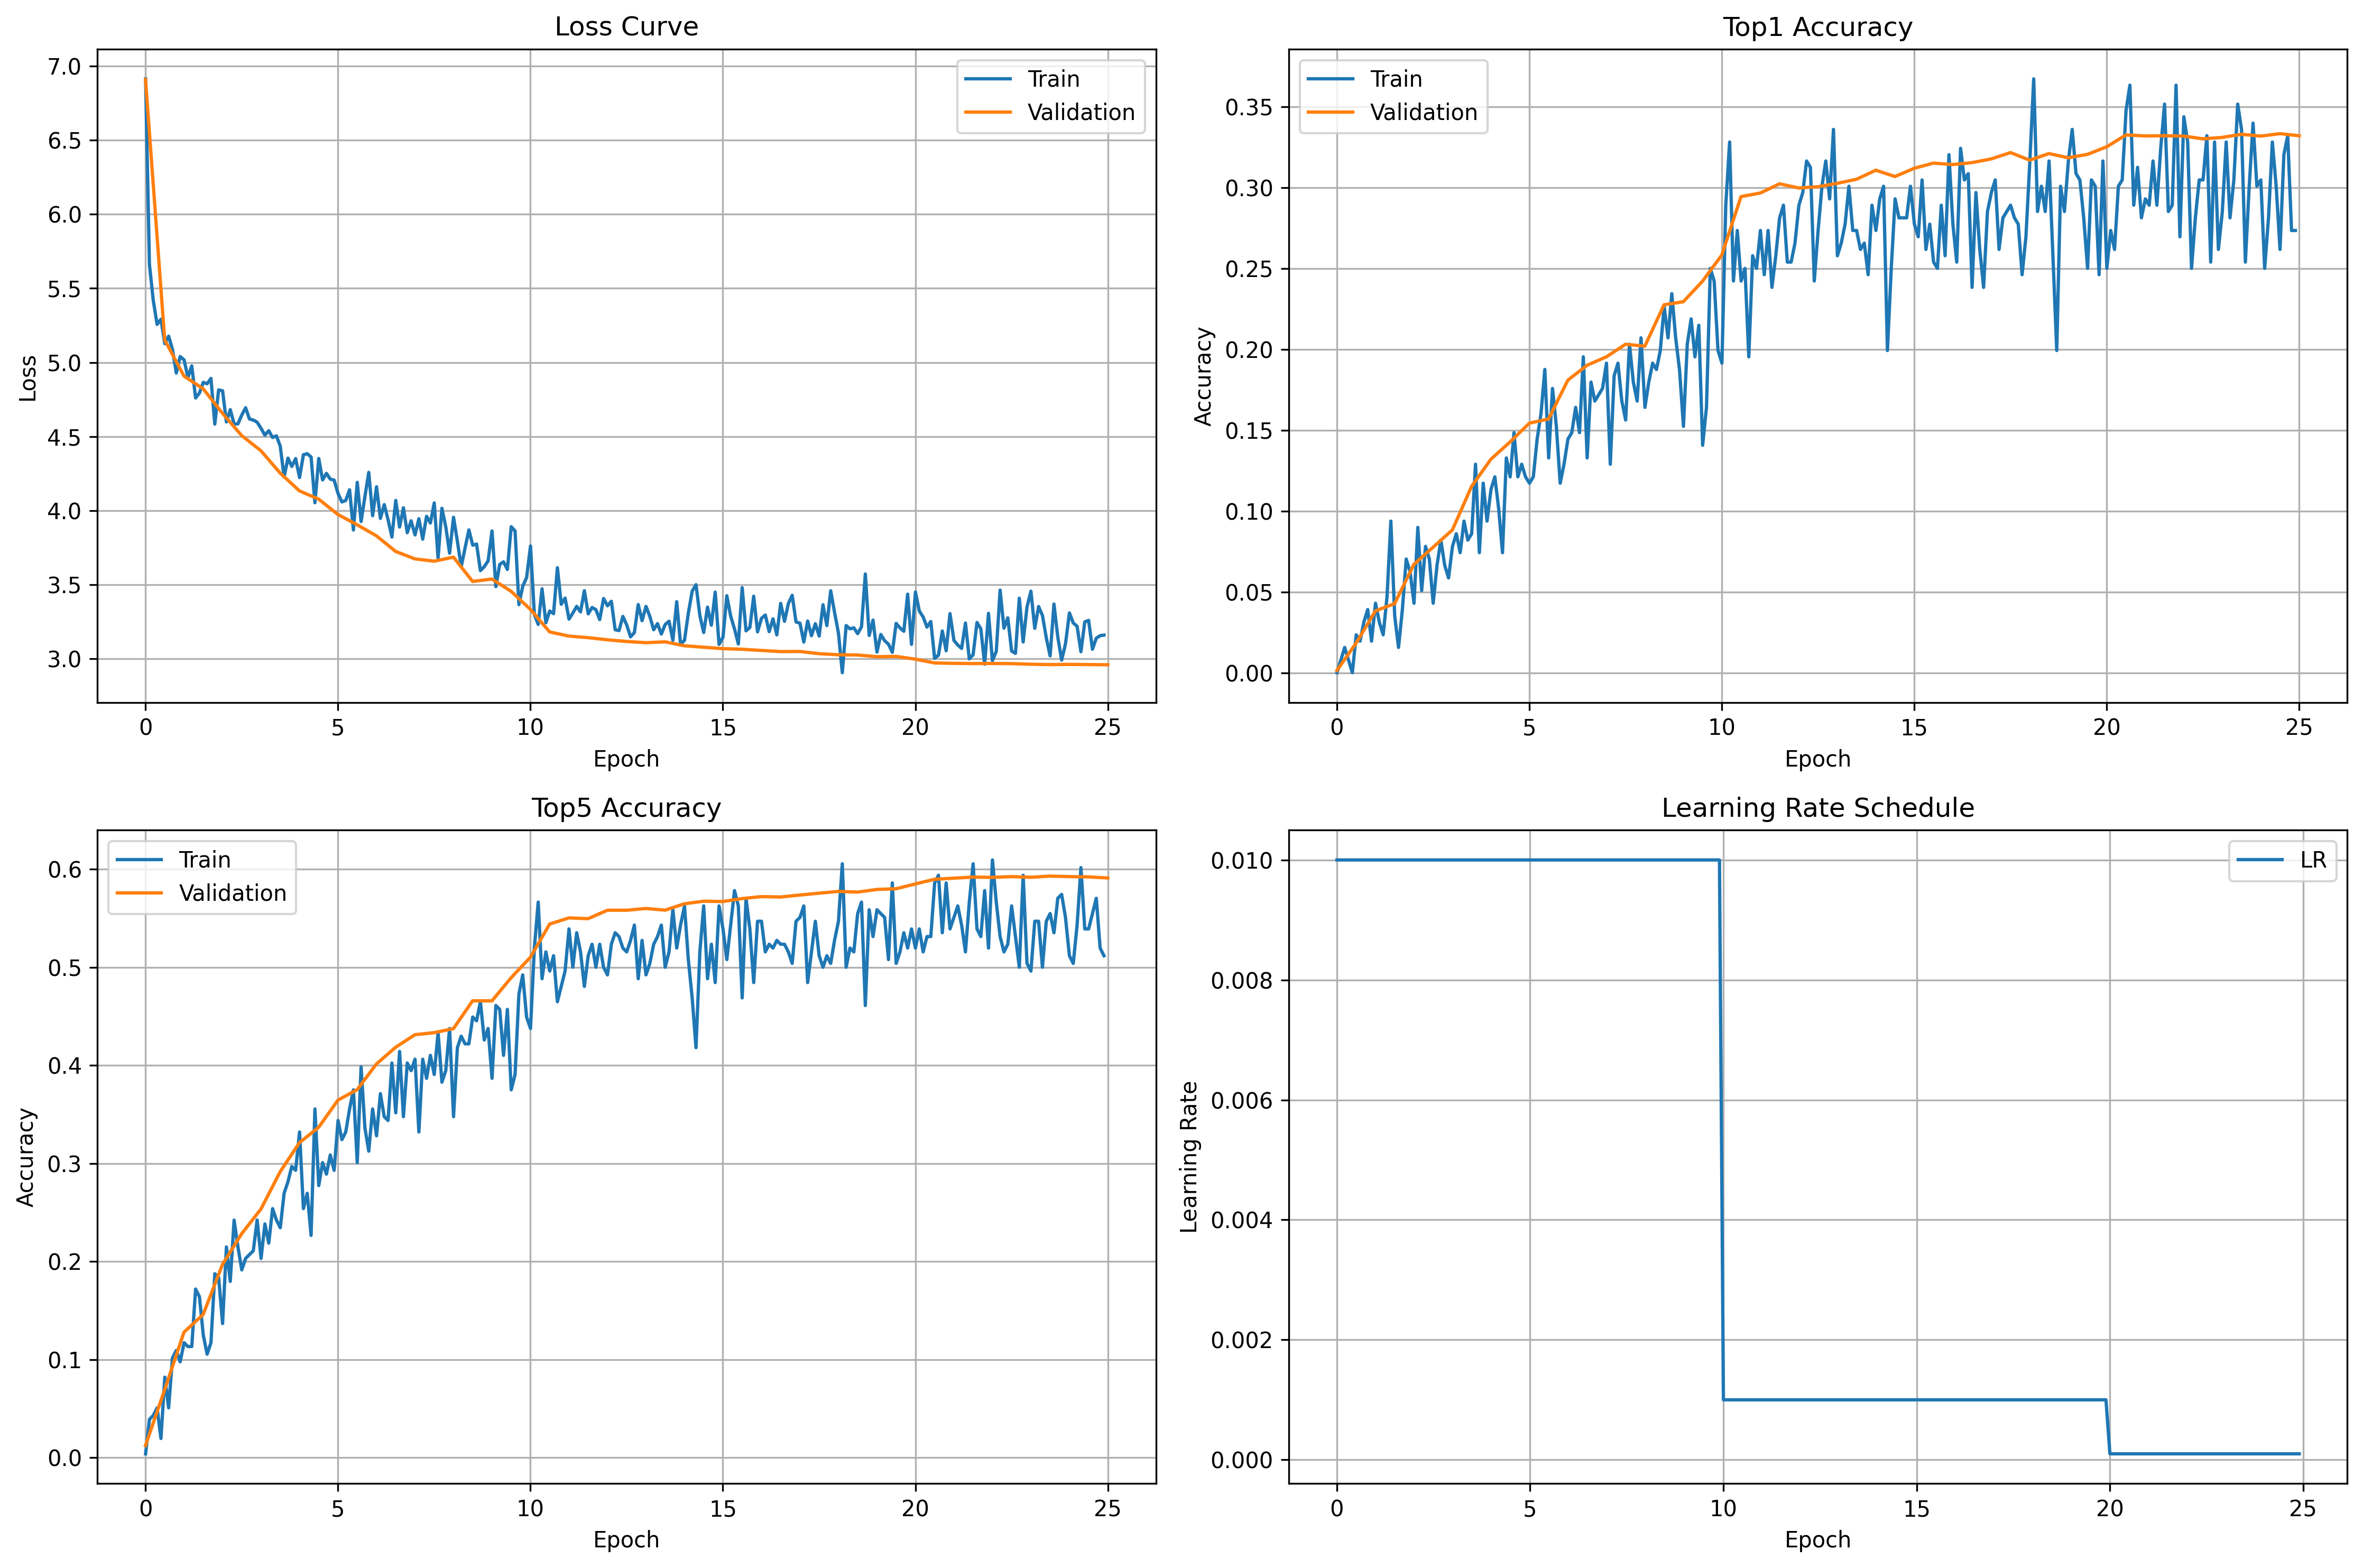
\includegraphics[width=0.9\linewidth]{cornet-z.png}
	\caption{CORnet-Z训练数据变化图}
	\label{f.zzxt}
\end{figure}

\begin{figure}[hbt]
	\centering
	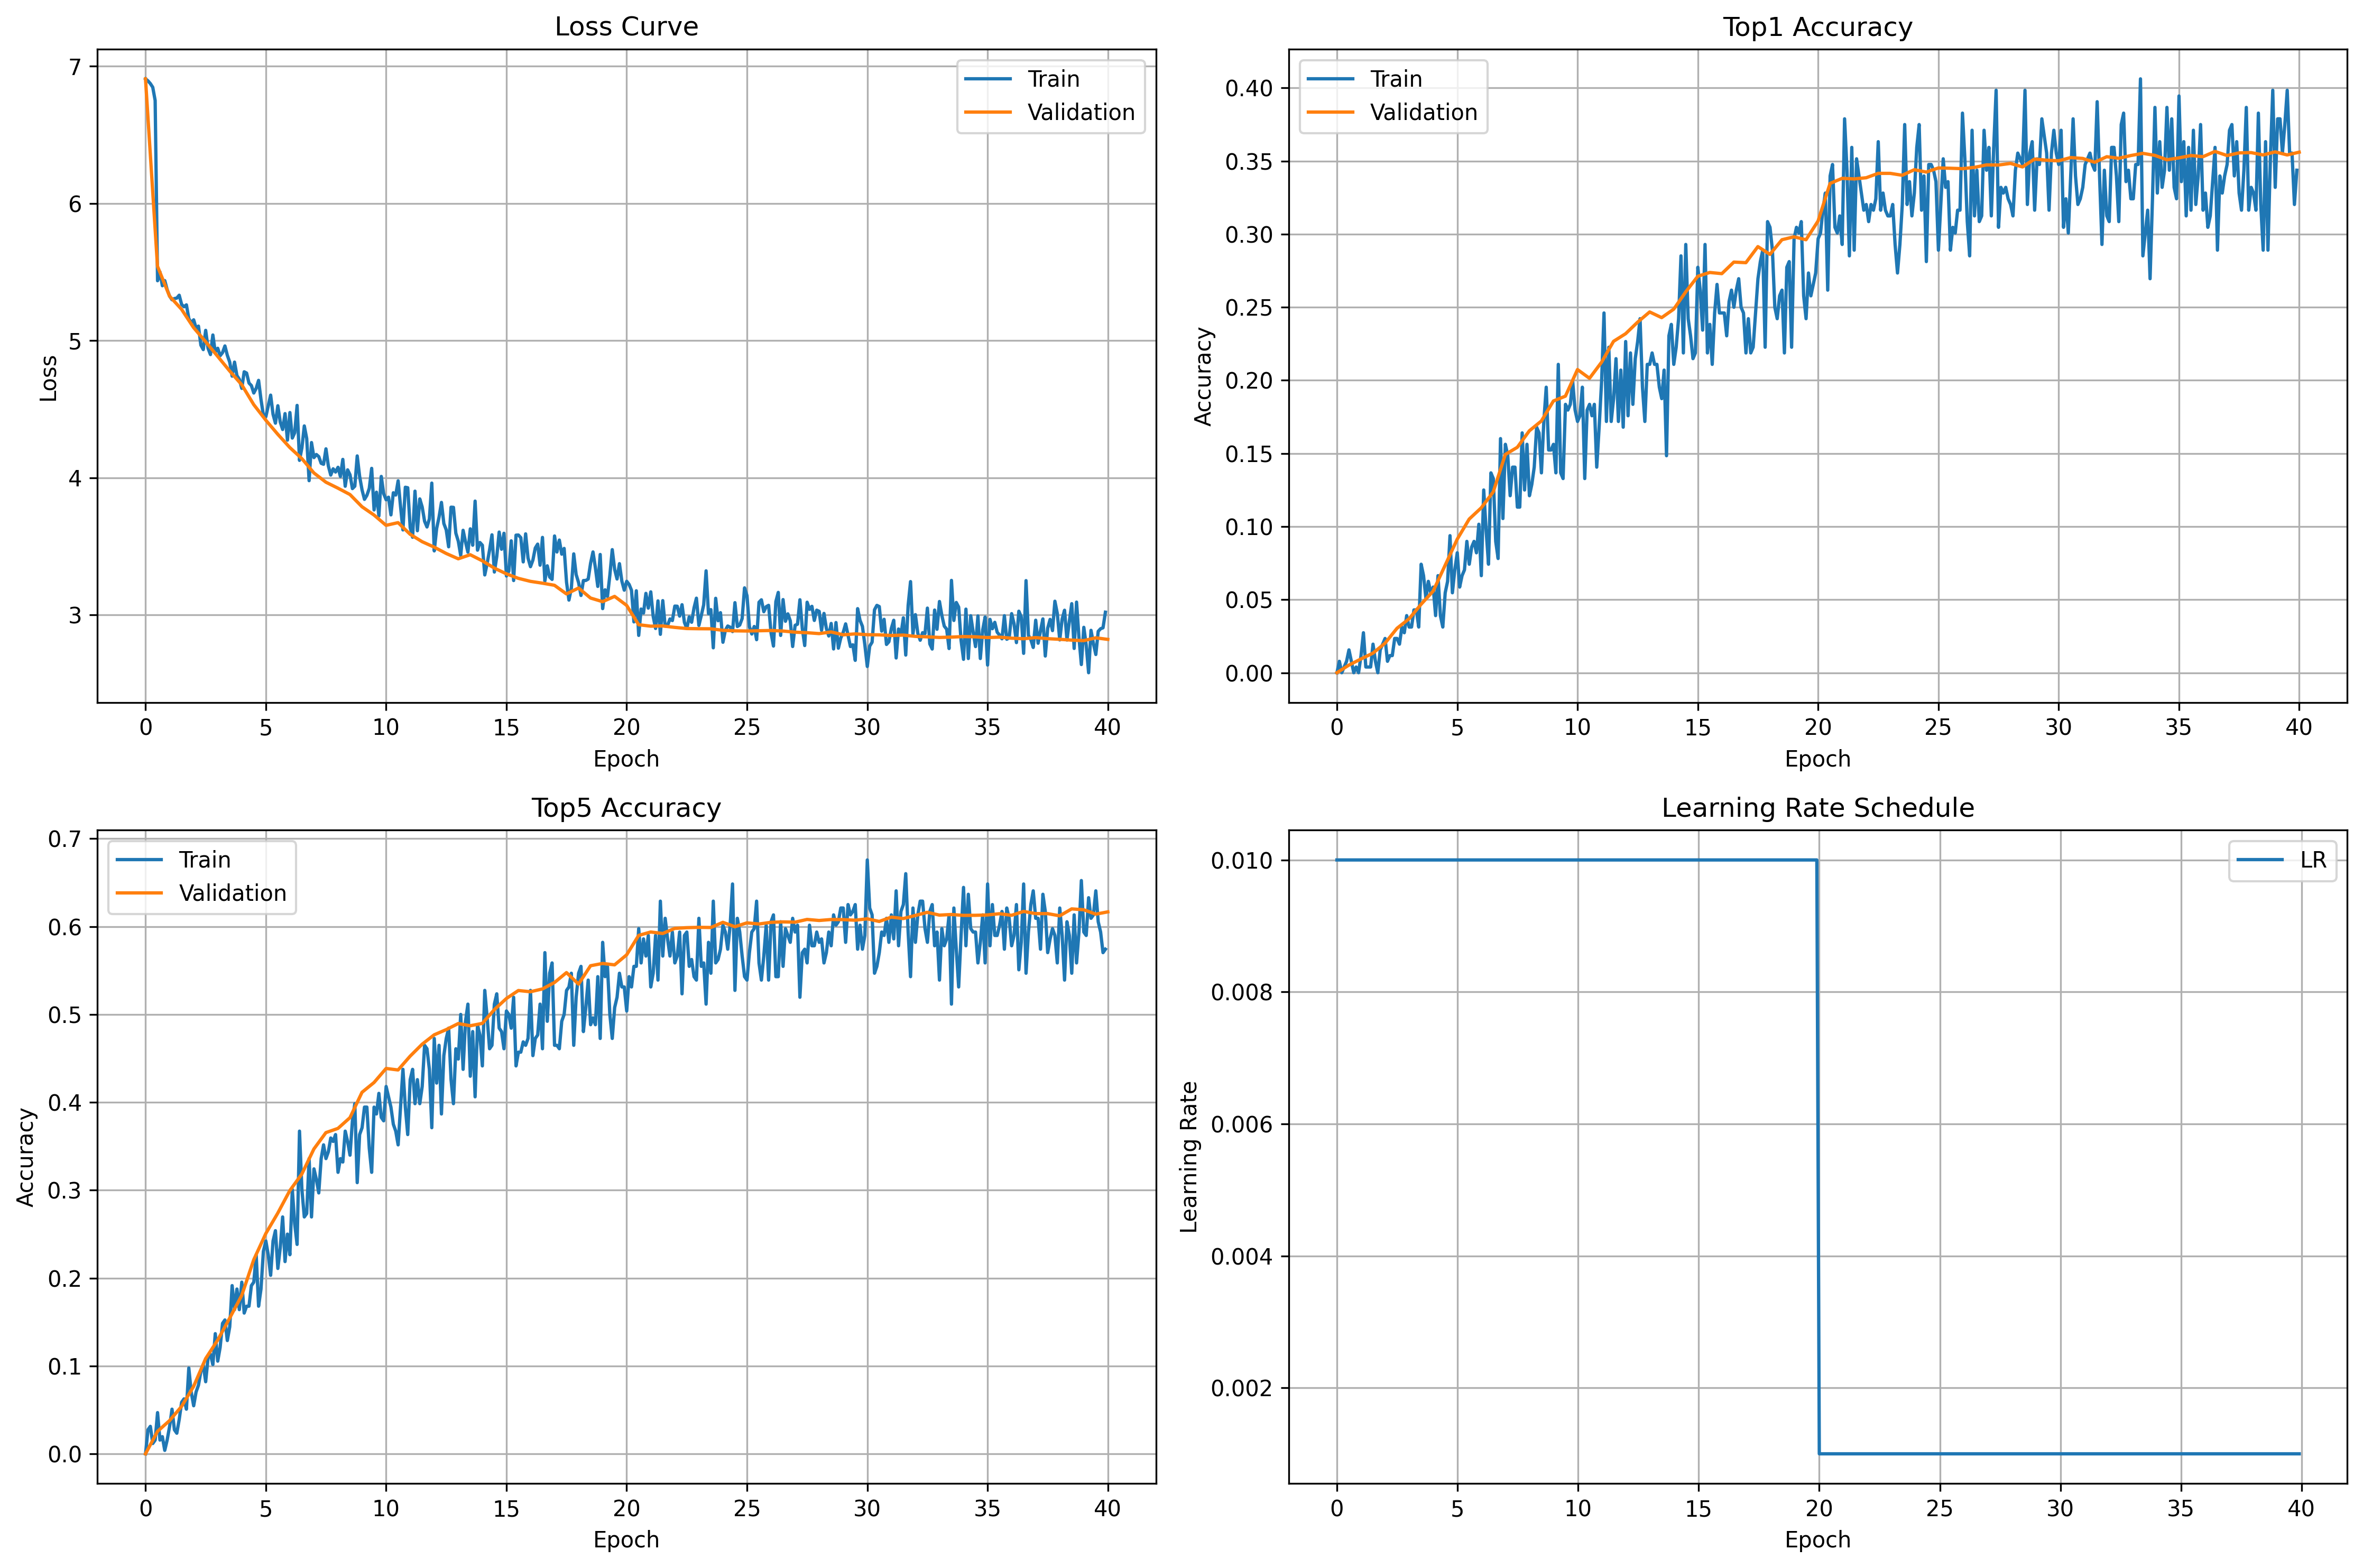
\includegraphics[width=0.9\linewidth]{cornet-z-SE.png}
	\caption{CORnet-Z+SE训练数据变化图}
	\label{f.zsezxt}
\end{figure}

总体来看,SE模块带来的Top-1提升幅度为2.33\%,Top-5提升为 2.51\%。虽然提升幅度有限,但考虑到模型结构变化极小,参数量变化可忽略,仍具有实际意义。尤其在训练集上的表现提升表明,注意力机制在训练早期能够加强对有效通道的识别,加快模型收敛速度。

\subsection{小结与分析}

通道注意力机制使模型能够根据全局信息动态调整各通道的响应强度,提升了模型对关键特征的表达能力。训练曲线显示,SE模型在准确率、损失值、学习曲线平稳性等方面均优于原始模型,在保持网络结构轻量的前提下实现了性能上的小幅提升。

不过,相较于大幅度结构重构或多尺度融合模型,本研究采用的改进方式较为保守,性能提升有限。这一结果也说明,通道注意力机制更适合作为辅助增强模块,而非单独主导模型性能的关键因素。
